\chapter{Implementation of Wall Oscillation}
\section{Mathematical Formulation of Wall Oscillation}
The wall oscillation model is applied along the streawise x-direction as shown by figure~\ref{fig:wall_oscill}.
\begin{figure}[h]
  \centering
  \scalebox{0.5}{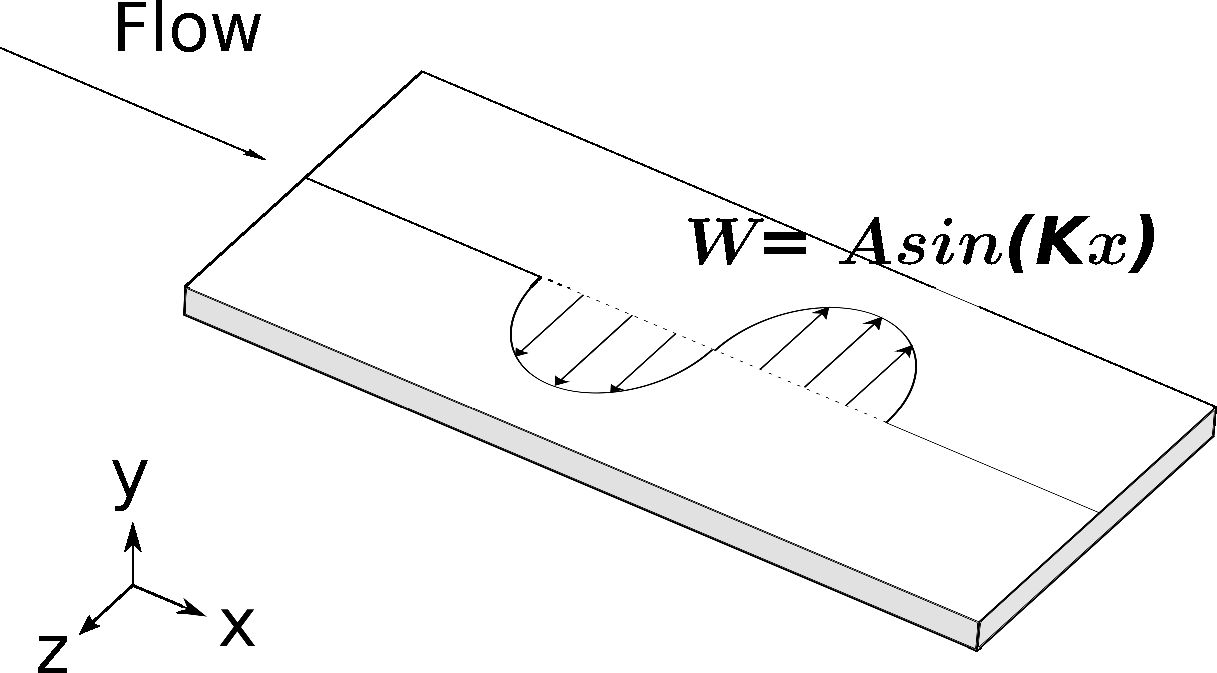
\includegraphics{figures/wall_oscill.pdf}}
  \caption{Wall oscillation model}
  \label{fig:wall_oscill}
\end{figure}
Since the wall oscillation only occurs on particular region, a profile function $f(x)$ is inserted to the wall oscillation model to act as a filter. The complete mathematical formulation of the wall oscillation can be seen in equation~\ref{eq:wall_oscill}.
\begin{equation}\label{eq:wall_oscill}
  w|_{y=0} = amp\cdot f(x)\cdot\sin (x_{omeg}x)
\end{equation}
With profile function $f(x)$ is formulated in equation~\ref{eq:prof_func}
\begin{equation}\label{eq:prof_func}
  f(x)=S\left(\frac{x-x_{start}}{x_{rise}}\right)-S\left(\frac{x-x_{end}}{x_{fall}}+1\right)
\end{equation}

The terms $amp,x_{start},x_{rise},x_{end},x_{fall}$ and $x_{omeg}$ are represented by the runtime parameter \emph{amp,xstart,xrise,xfall} and \emph{xomeg} respectively. Each terms description is given in table~\ref{tab:runtime}.
\begin{table}[h]
  \centering
  \begin{tabular}{|l|c|l|c|}\hline
    Runtime Parameter & Variable & Description & Data Type \\ \hline
    amp & wp1 & Maximum Amplitude & real \\
    xstart  & wpds1 & Start position of wall oscillation & real \\
    xend & wpds2 & End position of wall oscillation & real \\
    xrise & wpds3 & Rise length of wall oscillation & real \\
    xomeg & wpdds1 & Position variation & real \\ \hline
  \end{tabular}
  \caption{Correspondence between Runtime Parameter in bla.i and Variables in Subroutine rparambl}
  \label{tab:runtime}
\end{table}

$S(x)$ is a ''continuous'' step function which can be formulated in equation~\ref{eq:step_func}.
\begin{equation} \label{eq:step_func}
  S(x) = \left\{ 
    \begin{array}{lr}
      0, & x \leq 0 \\
      1/\left(1/1+e^{(1/(x-1)+1/x)}\right), & 0 < x < 1 \\
      1, & x \geq 1
    \end{array}
  \right.
\end{equation}
Schematic of function $S(x)$ is shown in figure~\ref{fig:step_func}.
\begin{figure}[h]
  \centering
  \scalebox{0.7}{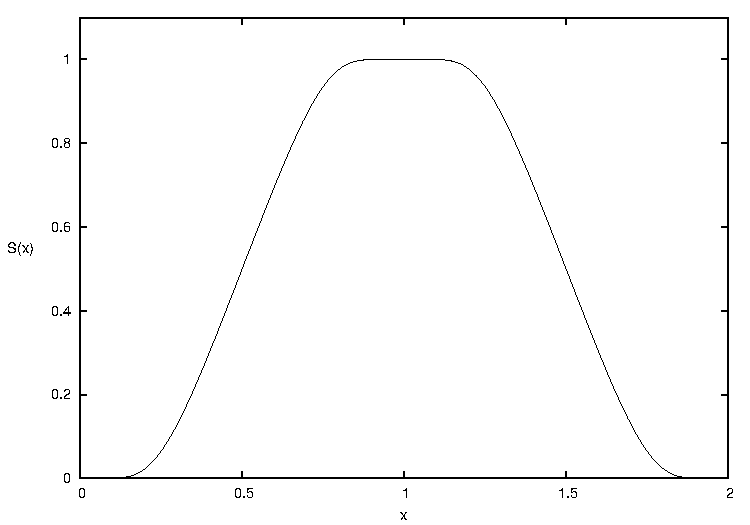
\includegraphics{figures/fx.pdf}}
  \caption{Schematic picture of function $S(x)$}
  \label{fig:step_func}
\end{figure}

\section{Computational Method}
The implementation of wall boundary condition to Simson is done by modification of the main program {\bf bla} and several subroutines, which are:
\begin{itemize}
\item {\bf cwallbc}, subroutine to set wall boundary condition,
\item {\bf rparambl}, subroutine used to link main program {\bf bla} and {\bf bla.i} that contains runtime parameters, and \item {\bf linearbl}, subroutine used to apply boundary condition
\end{itemize}

\subsection{Modification of subroutine rparambl}
Subroutine rparambl is used to read the runtime parameters stored in bla.i and relay the informations to bla as inputs needed during simulation. When new boundary conditions or variables are declared in cwallbc, the same boundary conditions and new variable need to be declared in rparambl as well.

Implementation of the new boundary layer model is done by setting a new value to wbci ($wbci = 4$). By setting a new value to wbci, a new boundary layer model is created in Simson. Other change done in rparambl is the initialization of new variables. These variables are runtime parameters needed by bla as inputs to simulate the new boundary layer condition. The list of new parameters declared in rparambl is available in table~\ref{tab:runtime}. Detail changes of subroutine rparambl is explained in appendix~\ref{app:bla_change}. The value of both wbci and new variables are assigned in bla.i as runtime parameters.
 
\subsection{Modification of subroutine cwallbc}
Subroutine cwallbc is used to set the boundary condition in Simson. Since the wall oscillation model is residing in cwallbc, the subroutine has been changed substantially. To implement the wall oscillation model, new variables are declared in cwallbc, which are: \emph{dnx, fstcm denc, r, xst, xen, imin, xendc, i, etc}. Some variables declared in last project ($wbci = 3$) are also included in the formulation, which are: \emph{walloscur, walloscui, walloscwr,and walloscwi}. Variables exist in original code, \emph{alfa} and \emph{beta}, are also included.

The next changes in cwallbc subroutine is the generation of the $w|_{y=0}$, which is represented by the variables \emph{wlwr} and \emph{wlwi}. Previous project ($wbci = 3$) manage to utilize the existing code from $wbci = 1$ successfully. However the same result could not be produce when used in the new wall oscillation model. When the existing code is applied to the new wall oscillation model, the resulting graphic show the there are discontinuities in the middle of the computational box. The discontinuity is caused by the generation of fringe function in the odd and even space respectively. Therefore, a difference approach is used to apply the wall oscillation model to the boundary condition. The major changes done in the new approach is the conversion of \emph{xstart} and \emph{xend} to channel code. 

Although previous project's approach could not be used for generation of $w|_{y=0}$, the transformation of variables \emph{wlwr} and \emph{wlwi} from real to half complex in x-directions is done by using the code from previous project. The same code is also used to do the normalization of variables \emph{wlwr} and \emph{wlwi}. The detail of all of the change in subroutine cwallbc is given in appendix~\ref{app:bla_change}.

\subsection{Modification of subroutine linearbl}
The boundary conditions are located in subroutine linearbl. The changes done In linearbl, different boundary condition are set on even/odd points and setting new boundary conditions for wavenumber zero. The detail of change is listed in appendix~\ref{app:bla_change}.

\subsection{Modification of main program bla} 
Main program bla is the main program where the operation of all subroutines are combined. The implementation of wall oscillation model to Simson requires some changes in main program bla as well. These changes are the declaration of new variables used in subroutine cwallbc and linearbl, which are wlwr, wlwi, walloscur, walloscui, wallloswr and walloscwi for all oscillation as a global variable. 

\section{Testing of Wall Oscillation}
To ensure the validity of the code, a test is performed to check the wall oscillation profile. Since no data will be collected during the test, the simulations are done in small scale. The size of the computational box is given by: $xl=112$, $yl=34$ and $zl=16$ which are set in \emph{bls.i}. The spectral number for \emph{x, y} and \emph{z}-direction is given by $nx =120, ny=61 \mbox{ and } nz=48$ which are set in \emph{par.f}. These parameters are the resolutions of the simulation.

The test simulations are performed in four cases according to the location of the wall oscillations. The first case is done with $xstart = 0$ and $xend = 40$, the second case is done with $xstart=40$ and $xend=80$, third case is done with $xstart=80$ and $xend = 112$ and the last case is done with $xstart = 0$ and $xend = 112$. All simulations are done with $xomeg = 0.38$, $xrise=20$, $xfall=20$ and $amp=0.5$.

The results of the test simulations can be seen in figure~\ref{fig:w(f(x))-test}. Since the test is done to test the wall oscillation profile, the simulation results are plotted as $w$ component as function of $x$ with $y=0$ ($w(f(x))|_{y=0}$).

\begin{figure}[!h]
  \centering
  \subfloat[]{\label{fig:w(f(x))-1}\scalebox{0.7}{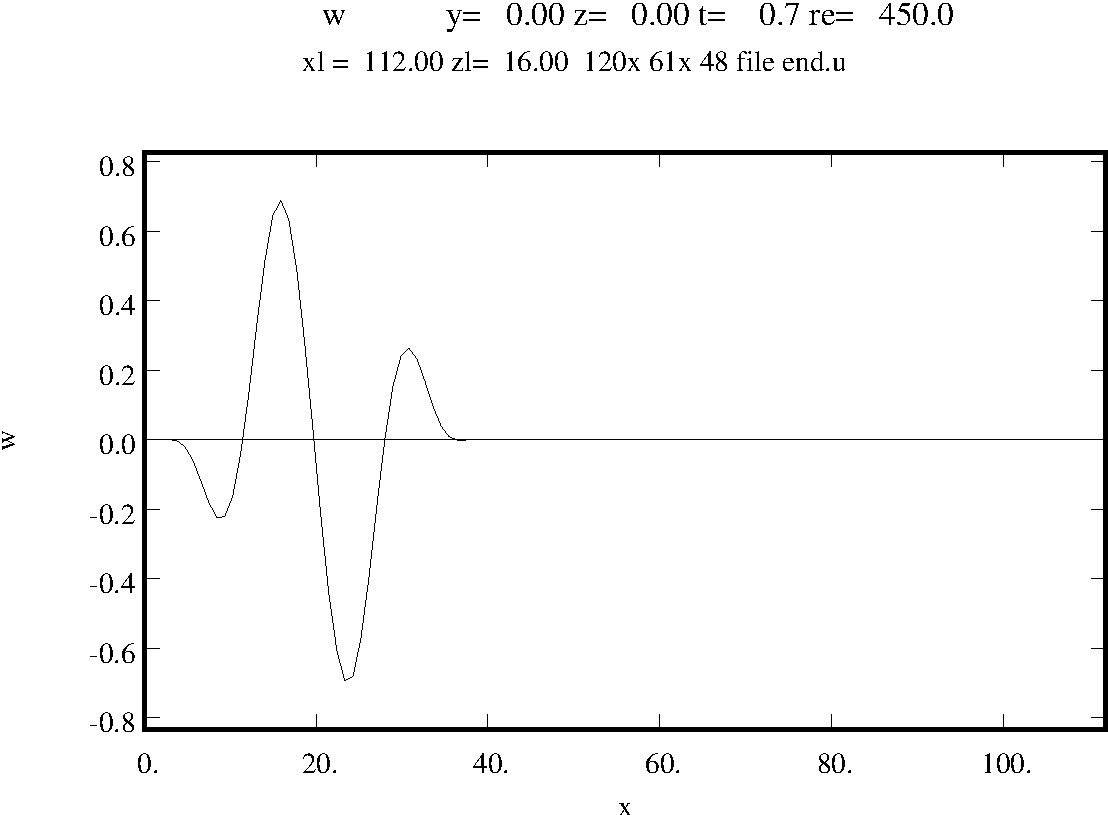
\includegraphics{figures/w(f(x))-1.pdf}}} \\
  \subfloat[]{\label{fig:w(f(x))-2}\scalebox{0.7}{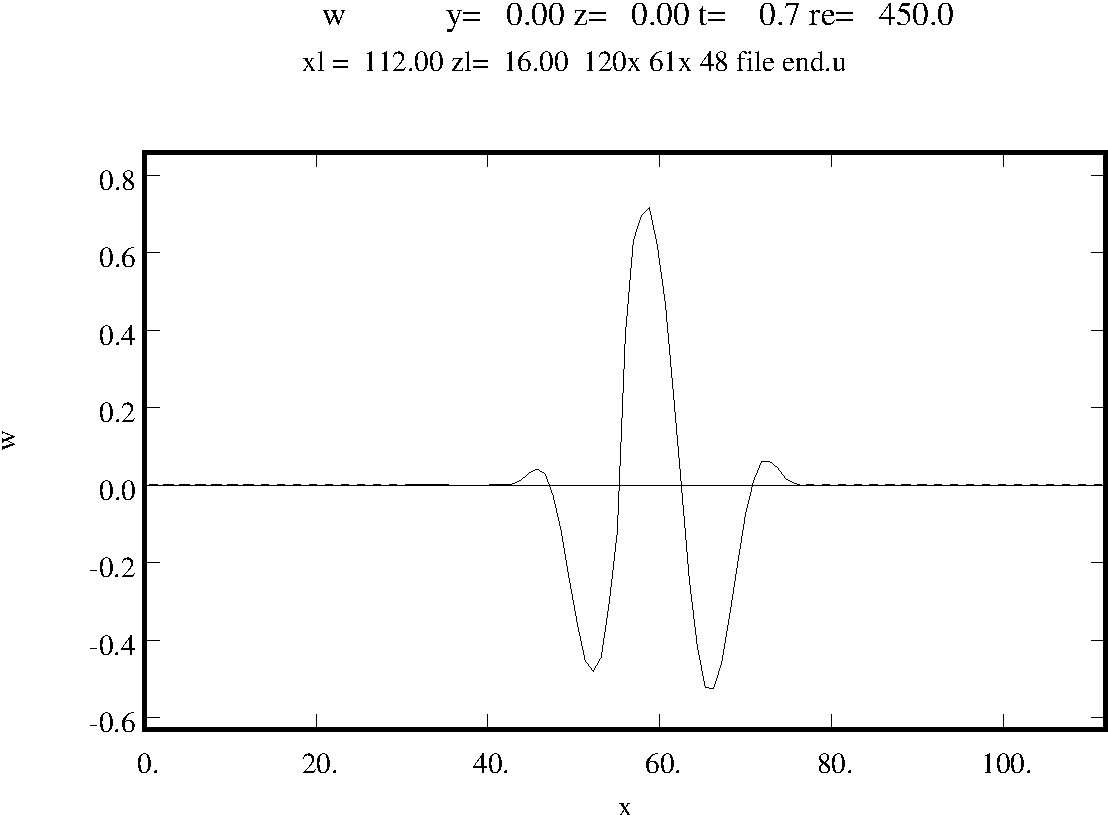
\includegraphics{figures/w(f(x))-2.pdf}}}
  \caption{Two dimensional contour plot of wall oscillation tested in various region at $y=0$: (a) $w(f(x))|_{y=0} \mbox{ at } xstart = 0 \mbox{ and } xend = 40$, (b) $w(f(x))|_{y=0} \mbox{ at } xstart = 40 \mbox{ and } xend = 80$, (c) $w(f(x))|_{y=0} \mbox{ at } xstart = 80 \mbox{ and } xend = 112$}
  \label{fig:w(f(x))-test}
\end{figure}

\begin{figure}[!h]
\ContinuedFloat
\centering
   \subfloat[]{\label{fig:w(f(x))-3}\scalebox{0.7}{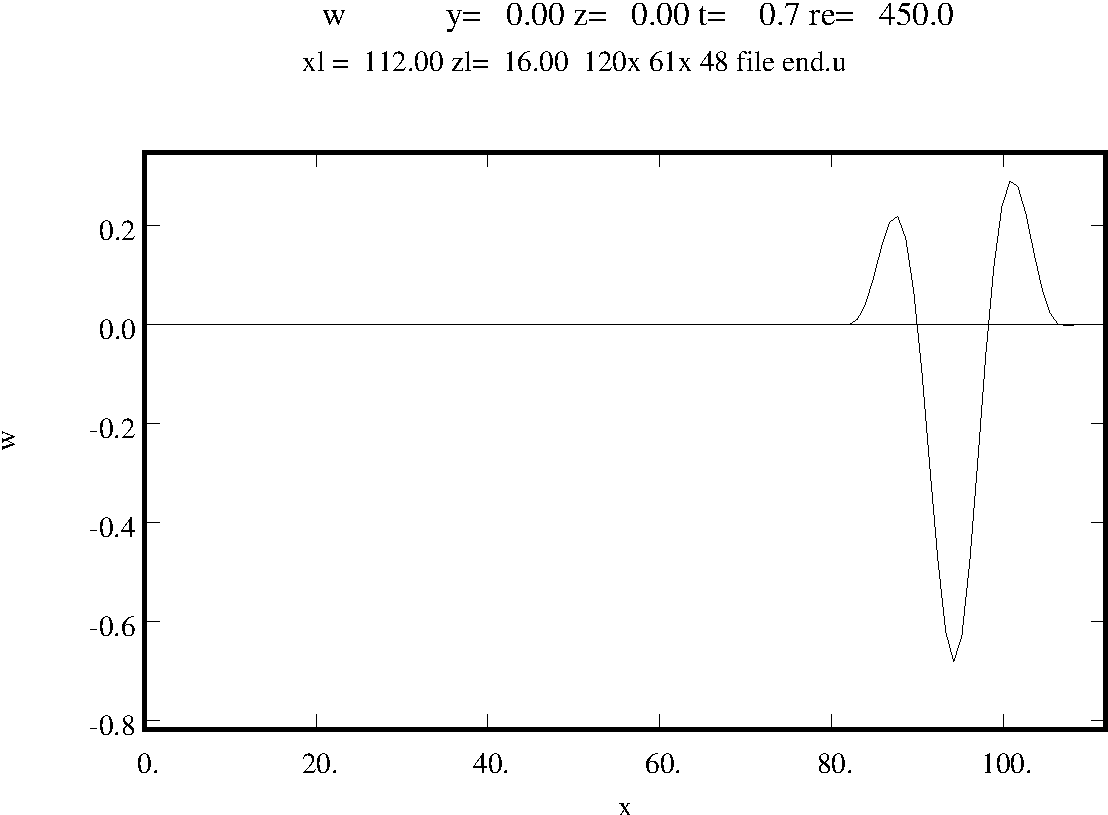
\includegraphics{figures/w(f(x))-3.pdf}}}\\
   \subfloat[]{\label{fig:w(f(x))-4}\scalebox{0.7}{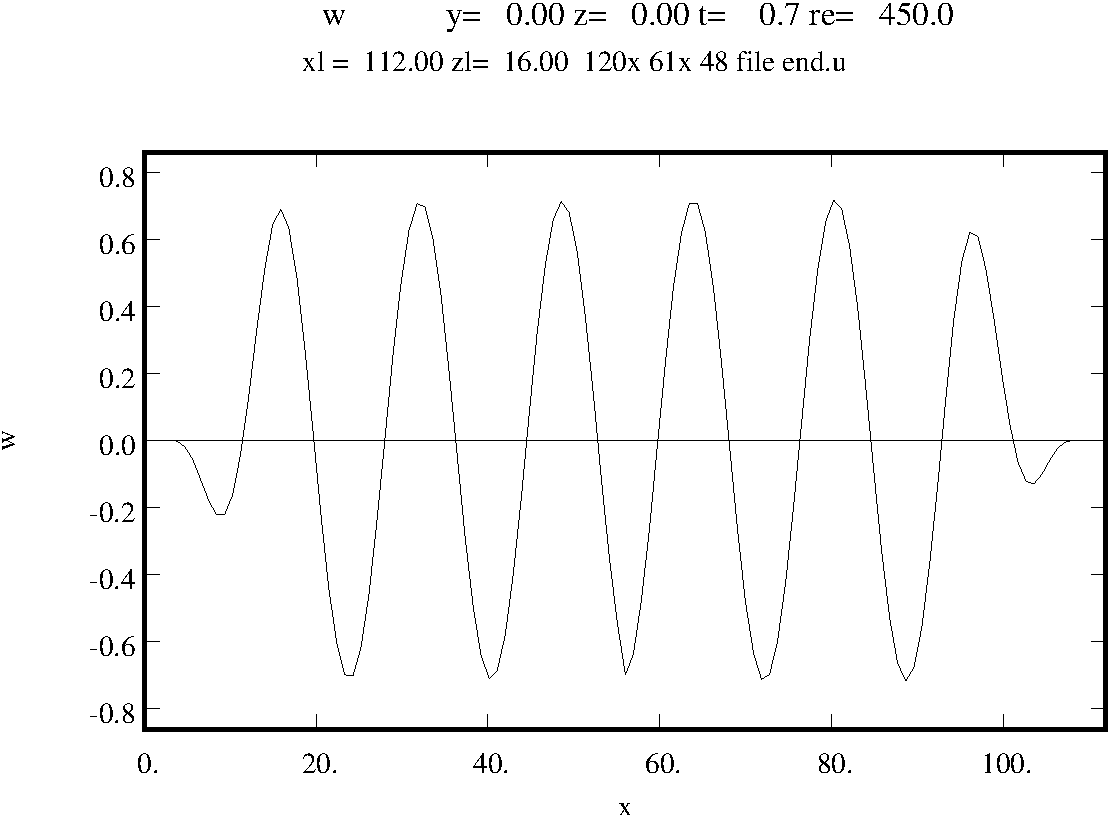
\includegraphics{figures/w(f(x))-4.pdf}}}
   \caption{Two dimensional contour plot of wall oscillation tested in various region at $y=0$: (a) $w(f(x))|_{y=0} \mbox{ at } xstart = 0 \mbox{ and } xend = 40$, (b) $w(f(x))|_{y=0} \mbox{ at } xstart = 40 \mbox{ and } xend = 80$, (c) $w(f(x))|_{y=0} \mbox{ at } xstart = 80 \mbox{ and } xend = 112$, (d)  $w(f(x))|_{y=0} \mbox{ at } xstart = 0 \mbox{ and } xend = 112$}
 \end{figure}

\section{Simulation Parameters}
For comparison purpose, the simulation's parameters used are similar to the parameters used in previous final year project~\cite{indra}. The parameters are listed in the table~\ref{tab:params}.
\begin{table}[h]
  \centering
  \begin{tabular}[h]{l c}
    \hline\hline
    Parameters & Value\\
    \hline
    $x_{start}$ & 250.0 \\
    $x_{end}$ & 482.7 \\
    $Re$ & 400 \\
    \hline
  \end{tabular}
  \caption{Simulation parameters}
  \label{tab:params}
\end{table}